\documentclass{article}
\usepackage[margin=0.75in]{geometry}
\usepackage{tikz}
\usetikzlibrary{positioning,arrows.meta}
\usepackage{tcolorbox}
\usepackage{fontawesome5}
\usepackage{xcolor}

\newcommand{\benchmark}{ChemChain}

\begin{document}

\section*{Chemistry Diagram: Before \& After Comparison}

\subsection*{ORIGINAL (Current Version)}

\begin{tcolorbox}[
    title=\textbf{Chemistry: Reaction Cascade} \hfill {\small\colorbox{teal!20}{Medium} \quad 9 steps},
    colframe=teal!70!black,
    colback=teal!3,
    boxrule=0.8pt,
    width=\textwidth
]
\small
\begin{tikzpicture}[remember picture, overlay]
    \node[opacity=0.08, anchor=east] at ([xshift=-0.3cm, yshift=0cm]current page.east) {\Huge\faFlask};
\end{tikzpicture}

\textbf{Dependency graph:}
\begin{center}
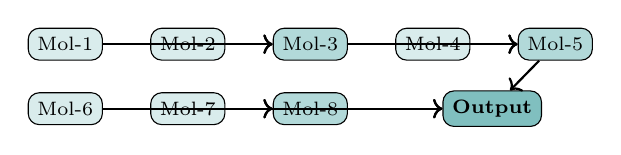
\begin{tikzpicture}[node distance=0.6cm, every node/.style={font=\scriptsize}]
    \node[draw, rounded corners, fill=teal!15] (m1) {Mol-1};
    \node[draw, rounded corners, fill=teal!15, right=of m1] (m2) {Mol-2};
    \node[draw, rounded corners, fill=teal!30, right=of m2] (m3) {Mol-3};
    \node[draw, rounded corners, fill=teal!15, right=of m3] (m4) {Mol-4};
    \node[draw, rounded corners, fill=teal!30, right=of m4] (m5) {Mol-5};
    \node[draw, rounded corners, fill=teal!15, below=0.4cm of m1] (m6) {Mol-6};
    \node[draw, rounded corners, fill=teal!15, right=of m6] (m7) {Mol-7};
    \node[draw, rounded corners, fill=teal!30, right=of m7] (m8) {Mol-8};
    \node[draw, rounded corners, fill=teal!50, right=1.2cm of m8] (out) {\textbf{Output}};

    \draw[->, thick] (m1) -- (m3);
    \draw[->, thick] (m2) -- (m3);
    \draw[->, thick] (m3) -- (m5);
    \draw[->, thick] (m4) -- (m5);
    \draw[->, thick] (m6) -- (m8);
    \draw[->, thick] (m7) -- (m8);
    \draw[->, thick] (m5) -- (out);
    \draw[->, thick] (m7) -- (out);
    \draw[->, thick] (m8) -- (out);
\end{tikzpicture}
\end{center}

\vspace{-0.3cm}
\begin{tabular}{@{}p{0.48\textwidth}p{0.48\textwidth}@{}}
\textit{Sample step (Subproblem 3):} React Mol-1 + Mol-2 in THF at room temp. Predict major product. &
\textit{Final step:} Count hydrogens in Mol-5, Mol-7, Mol-8. \\
\end{tabular}

\vspace{0.2cm}
\hfill \textbf{Answer:} \texttt{[19, 15, 23]}
\end{tcolorbox}

\textbf{Issues:} Cramped spacing, unclear flow direction, subtle color differences, arrows cross awkwardly

\vspace{1cm}

\subsection*{IMPROVED VERSION 2 (Recommended)}

\begin{tcolorbox}[
    title=\textbf{Chemistry: Reaction Cascade} \hfill {\small\colorbox{teal!20}{Medium} \quad 9 steps},
    colframe=teal!70!black,
    colback=teal!3,
    boxrule=0.8pt,
    width=\textwidth
]
\small
\begin{tikzpicture}[remember picture, overlay]
    \node[opacity=0.05, anchor=east] at ([xshift=-0.4cm, yshift=0.2cm]current page.east) {\Huge\faFlask};
\end{tikzpicture}

\textbf{Dependency graph:}
\begin{center}
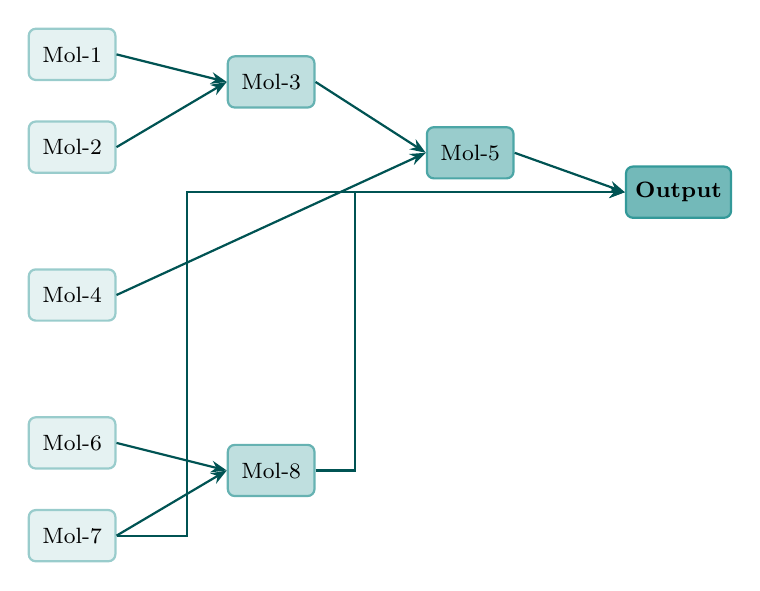
\begin{tikzpicture}[
    node distance=0.8cm and 1.1cm,
    every node/.style={font=\footnotesize},
    mol/.style={draw, rounded corners=2.5pt, minimum width=1.1cm, minimum height=0.65cm, thick},
    lvl0/.style={mol, fill=teal!10, draw=teal!40},
    lvl1/.style={mol, fill=teal!25, draw=teal!60},
    lvl2/.style={mol, fill=teal!40, draw=teal!70},
    lvl3/.style={mol, fill=teal!55, draw=teal!80, font=\footnotesize\bfseries},
    arrow/.style={-{Stealth[length=2mm]}, thick, teal!65!black}
]
    % Column 1: Initial molecules
    \node[lvl0] (m1) {Mol-1};
    \node[lvl0, below=0.5cm of m1] (m2) {Mol-2};
    \node[lvl0, below=1.2cm of m2] (m4) {Mol-4};
    \node[lvl0, below=1.2cm of m4] (m6) {Mol-6};
    \node[lvl0, below=0.5cm of m6] (m7) {Mol-7};

    % Column 2: First reactions
    \node[lvl1, right=1.4cm of m1.east, yshift=-0.35cm] (m3) {Mol-3};
    \node[lvl1, right=1.4cm of m6.east, yshift=-0.35cm] (m8) {Mol-8};

    % Column 3: Second reaction
    \node[lvl2, right=1.4cm of m3.east, yshift=-0.9cm] (m5) {Mol-5};

    % Column 4: Final output
    \node[lvl3, right=1.4cm of m5.east, yshift=-0.5cm] (out) {Output};

    % Draw arrows
    \draw[arrow] (m1.east) -- (m3.west);
    \draw[arrow] (m2.east) -- (m3.west);
    \draw[arrow] (m3.east) -- (m5.west);
    \draw[arrow] (m4.east) -- (m5.west);
    \draw[arrow] (m6.east) -- (m8.west);
    \draw[arrow] (m7.east) -- (m8.west);
    \draw[arrow] (m5.east) -- (out.west);
    \draw[arrow] (m8.east) -| ([xshift=0.5cm]m8.east) |- (out.west);
    \draw[arrow] (m7.east) -| ([xshift=0.9cm]m7.east) |- (out.west);
\end{tikzpicture}
\end{center}

\vspace{0.1cm}
\begin{tabular}{@{}p{0.48\textwidth}p{0.48\textwidth}@{}}
\textit{Sample step (Subproblem 3):} React Mol-1 + Mol-2 in THF at room temp. Predict major product. &
\textit{Final step:} Count hydrogens in Mol-5, Mol-7, Mol-8. \\
\end{tabular}

\vspace{0.25cm}
\hfill \textbf{Answer:} \texttt{[19, 15, 23]}
\end{tcolorbox}

\textbf{Improvements:} Better spacing (1.1-1.4cm), clear left-to-right flow, distinct color levels, cleaner arrow routing

\end{document}
